For at finde de grundlæggende specifikationer til systemet, skal problemet udspecificeres.  

Graf \ref{vandspild_graf_normal} viser et eksempel på hvordan temperaturændringerne forekommer, hvis det antages at vandspildet negligeres og temperaturen på røret derfor er lig med temperaturen i rummet. 
\\
\\
\begin{figure}[h!]
  \centering
  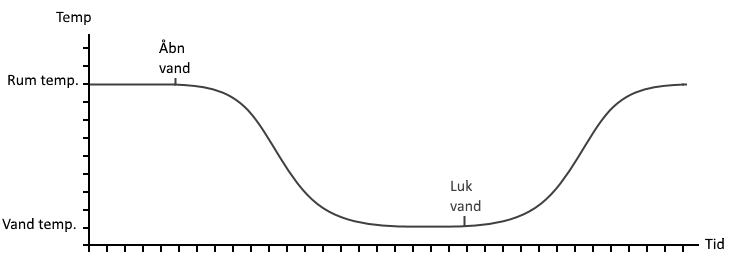
\includegraphics[width=1\textwidth]{figures/vandspild_graf_normal.png}
  \caption{Eksempel på vandtemperatur i vandrør når der åbnes og lukkes for vandet.}
  \label{vandspild_graf_normal}
\end{figure}
\\
\\
Tilførslen af nyt vand til huset ændrer rørets temperatur og derfor vil der forekomme temperatursvingninger, som målingen kan vise vandspildet ud fra. Graf \ref{vandspild_graf_spild} viser et teoretisk eksempel på temperaturændringer ved vandspild på et rør.
\newpage
På graf \ref{vandspild_graf_spild} ses hvordan hviletemperaturen på røret aldrig når temperaturen i rummet, da vandet aldrig ligger helt stille og derfor tilfører en konstant koldere temperatur.
\begin{figure}[h!]
  \centering
  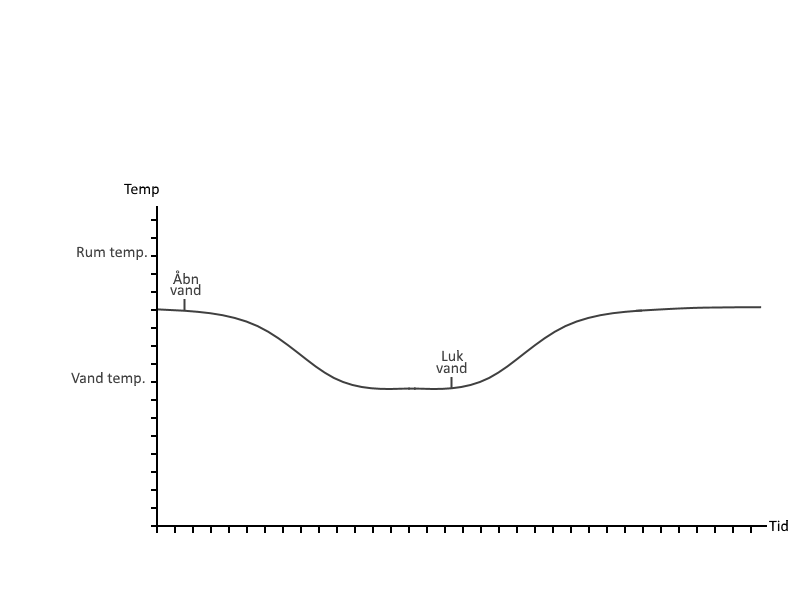
\includegraphics[width=1\textwidth]{figures/vandspild_graf_spild.png}
  \caption{Eksempel på vandtemperatur i vandrør når der åbnes og lukkes for vandet, når der er et vandspild.}
  \label{vandspild_graf_spild}
\end{figure}
\\
\\
Ud fra graferne \ref{vandspild_graf_normal} og \ref{vandspild_graf_spild}, ses en teoretisk forskel tydeligt. Det kan konkluderes at der er et problem, som ikke kan løses med regulering. Problemet skal i stedet løses med måleenheder som skal give kunden et overblik over omfanget af vandspild.
\\
\\
Produktet skal kunne overvåge vandspild uden at have regulerbare funktioner. Det skal kunne måle temperaturen i henholdvis overfladen på vandrøret og rummet. Endvidere skal det kunne sammenligne de to temperaturer.
\\
\\
Kravene for produktet er opstillet i det efterfølgende afsnit.     